\documentclass[a4paper, 12pt]{report}
\usepackage{cmap}
\usepackage[T2A]{fontenc}
\usepackage[utf8]{inputenc}
\usepackage[english,russian]{babel}
\usepackage{listings}
\usepackage{amsmath}
\usepackage{float}
\usepackage{csquotes}
\usepackage{graphicx}
\graphicspath{ {./images/} }
\usepackage{xcolor}
\definecolor{buzzlightyear}{HTML}{8757A5}
\definecolor{grass}{HTML}{738D06}
\definecolor{literal}{HTML}{F18A2B}
\definecolor{commentcolor}{HTML}{8E908B}

\lstdefinestyle{habrstyle}{
	backgroundcolor=\color{white},
	commentstyle=\color{commentcolor},
	keywordstyle=\bfseries\color{buzzlightyear},
	numberstyle=\tiny\color{commentcolor},
	stringstyle=\color{grass},
	basicstyle=\ttfamily\footnotesize,
	breakatwhitespace=false,         
    	breaklines=true,                 
   	captionpos=b,                    
    	keepspaces=true,                 
    	numbers=left,                    
    	numbersep=7pt,                  
    	showspaces=false,                
    	showstringspaces=false,
   	showtabs=false,                  
    	tabsize=3
}

\lstset{style=habrstyle}

\author{3530901/80201, Шелаев Н. Р.}
\title{Лабораторная работа № 12. GNU Radio.}
\date{\today}

\begin{document}
	\maketitle
	\tableofcontents
	\listoffigures

	\chapter{Цель работы}
	В этой работе мы поробуем достичь следующих целей:
	\begin{itemize}
        		\item разобраться в  проблемах искажения сигналов и \textquote{канальных} эффектах
        		\item определить этапы, необходимые для восстановления сигналов:
        		\begin{itemize}
            		\item временное восстановление сигналов
           		\item каналы с множеством путей
           		\item коррекция фазы и частоты
            		\item декодирование символов и упорядочивание битов
        		\end{itemize}
    	\end{itemize}
	
	Официально Windows не поддерживается, но Хорошие люди написали бинарные файлы для установки пакета GNU Radio на Windows. Были небольшие проблемы с установкой, но их удалось успешно преодолеть.
Вся работа была выполнена в версии GNU Radio 3.8 для Python 2.7 .
	
	\chapter{Передача сигнала}
	Первый этап построения канала передачи - передача сигнала \sloppy{\texttt{QPSK}}. \sloppy{\texttt{QPSK}}- это Quadrature Phase Shift Keying или \sloppy{\texttt{4PSK}}, или квадратурная фазовая модуляция. Эта модуляция использует созвездие из 4-х точек, размещённых ра равных расстояниях на окружности. На один передаваемый символ приходится 2 бита. Символы располагаются на этой окружности и имеют комплексные координаты. 
	
	Для генерации потока битов мы будем использовать блок модулятора Созвездия (\sloppy{\texttt{Constellation Modulator Block}} или \sloppy{\texttt{Constellaton Rect.Object}}). Этот объект позволяем нам определить, как кодируются символы. 

	Также нам потребуется генератор байтов со значениями от 0 до 255. 
	\begin{figure}[H]
		\centering
		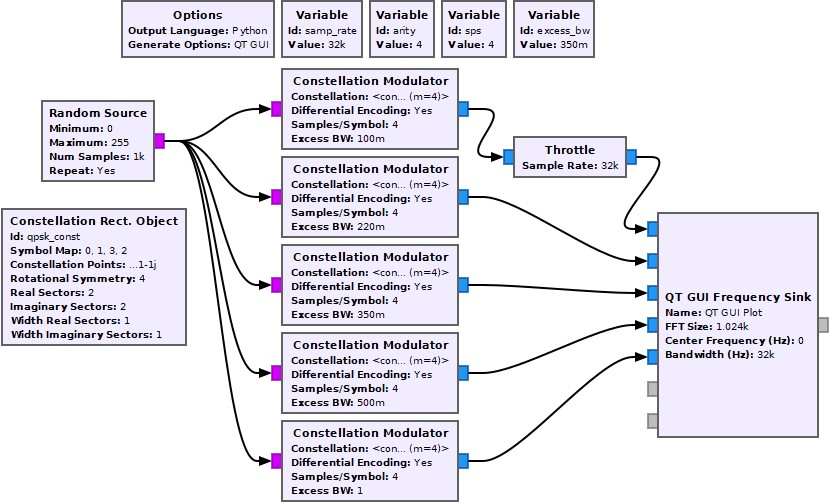
\includegraphics[width=1.0\textwidth]{1.jpg}
		\caption{Схема 1. \texttt{mpsk\_rrc\_rolloff.grc}}
		\label{fig:1}
	\end{figure}
	Здесь показаны различные значения избыточной пропускной способности. Типичные значения находятся в диапазоне от 0,2 (красный след) до 0,35 (зеленый след).
	\begin{figure}[H]
		\centering
		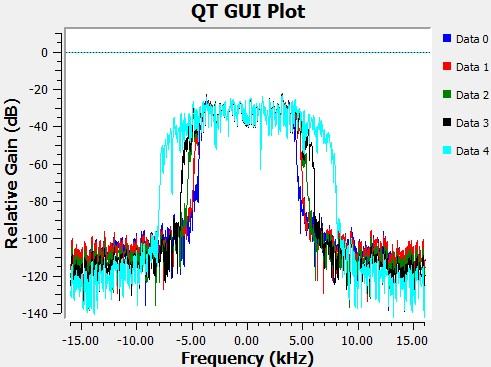
\includegraphics[width=1.0\textwidth]{2.jpg}
		\caption{Наблюдаемый результат}
		\label{fig:2}
	\end{figure}
	Следующая диаграмма передает созвездие QPSK. Он отображает передаваемый сигнал и принятый сигнал по времени, частоте и созвездии.
	\begin{figure}[H]
		\centering
		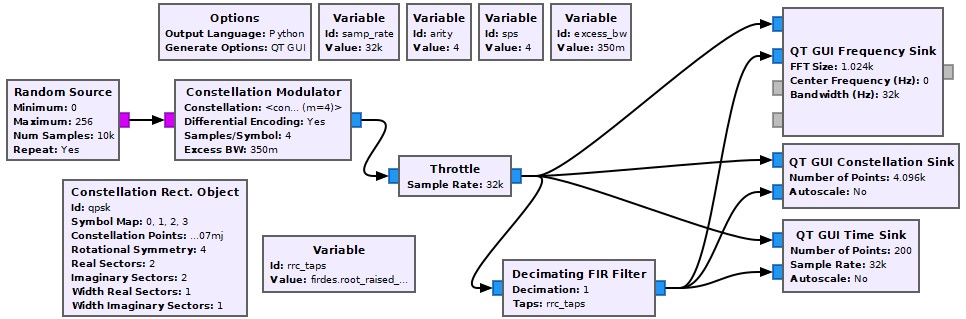
\includegraphics[width=1.0\textwidth]{3.jpg}
		\caption{Схема 2. \texttt{mpsk\_stage1.grc}}
		\label{fig:3}
	\end{figure}
	\begin{figure}[H]
		\centering
		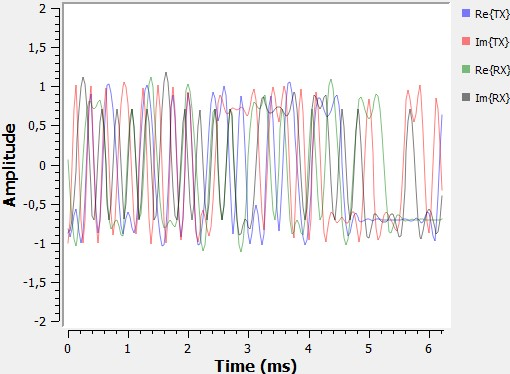
\includegraphics[width=1.0\textwidth]{4.jpg}
		\caption{Зависимость по времени}
		\label{fig:4}
	\end{figure}
	\begin{figure}[H]
		\centering
		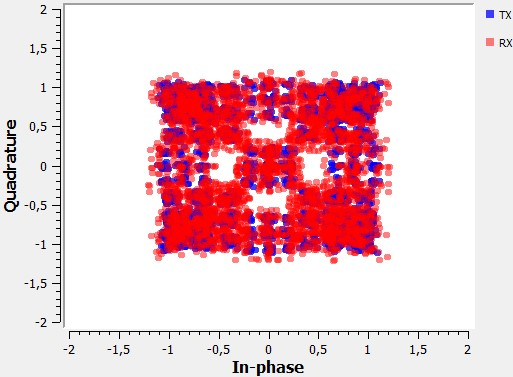
\includegraphics[width=1.0\textwidth]{5.jpg}
		\caption{Зависимость по фазе}
		\label{fig:5}
	\end{figure}
	\begin{figure}[H]
		\centering
		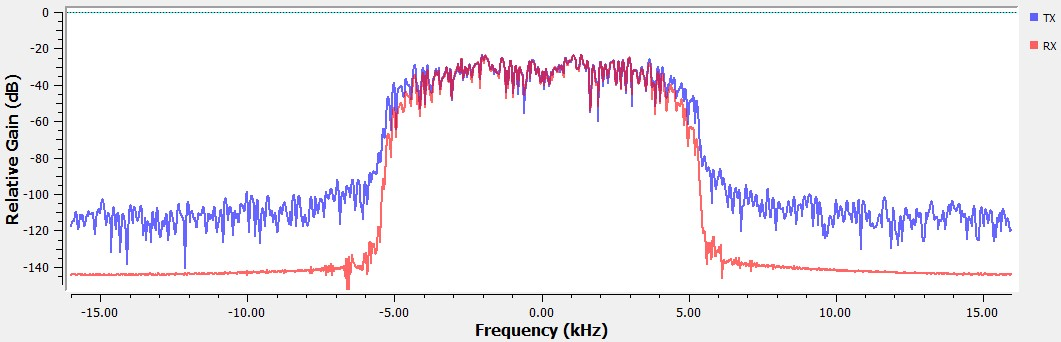
\includegraphics[width=1.0\textwidth]{6.jpg}
		\caption{Зависимость по частоте}
		\label{fig:6}
	\end{figure}
	На графике созвездия мы видим эффекты процесса предварительной выборки (создание 4 выборок на символ) и фильтрации. В этом случае \sloppy{\texttt{RRC}}-фильтр добавляет преднамеренную самоинтерференцию, известную как межсимвольная интерференция (\sloppy{\texttt{ISI}}). \sloppy{\texttt{ISI}} плохо влияет на принятый сигнал, потому что он размывает символы. Если использовать формирующий фильтр на передатчике, то сигнал выйдет за полосу пропускания нашего канала.
	
	Чтобы убрать \sloppy{\texttt{ISI}}, мы подключим на приемной стороне ещё один \sloppy{\texttt{RRC}}-фильтр. С помощью операции свертки на два \sloppy{\texttt{RRC}}-фильтра мы получаем поднятый косинусный фильтр, и на выходе приемника оказывается сигнал в форме косинусоидального импульса с минимальным значением \sloppy{\texttt{ISI}}.

	\chapter{Добавление искажений в канале}
	Сейчас мы рассмотрим так называемые \textquote{канальные} эффекты, которые искажают сигнал при его передаче от передатчика к приемнику.
	
	Добавим модель канала с помощью модуля \sloppy{\texttt{Channel Mode}}. Это базовый блок модели канала. 
	Этот канал позволит нам смоделировать несколько основных проблем при передаче сигнала. Первая проблема - шум в канале передачи (Аддитивный белый гауссовский шум). Мощность шума мы устанавливаем, регулируя значение напряжения шума модели канала. 
	
	Вторая проблема - разная частота синхронизации между приемником и передатчиком. Тактовая частота не может быть абсолютно точной и содержит некоторую погрешность. 
	
	С этой проблемой связана другая - идеальная точка выборки сигнала. Передатчик и приемник работают независимо друг от друга и на разных скоростях, поэтому идеальная точка выборки неизвестна.
	
	Следующая диаграмма позволяет нам изменять значение аддитивного шума, смещения частоты и времени.
	\begin{figure}[H]
		\centering
		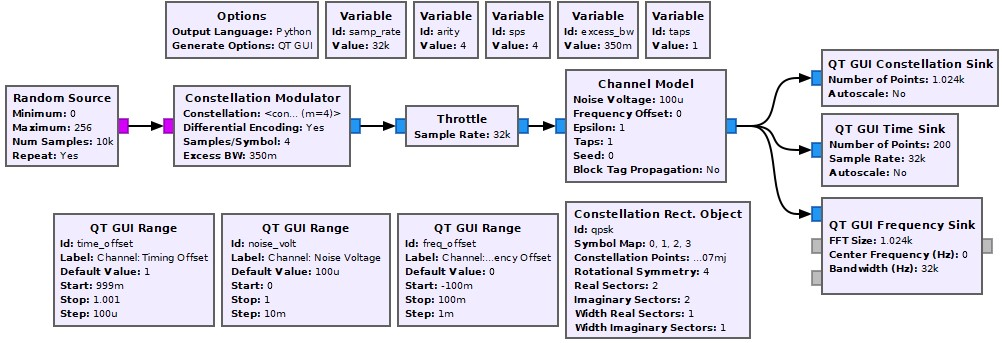
\includegraphics[width=1.0\textwidth]{7.jpg}
		\caption{Схема 3. \texttt{mpsk\_stage2.grc}}
		\label{fig:7}
	\end{figure}
	\begin{figure}[H]
		\centering
		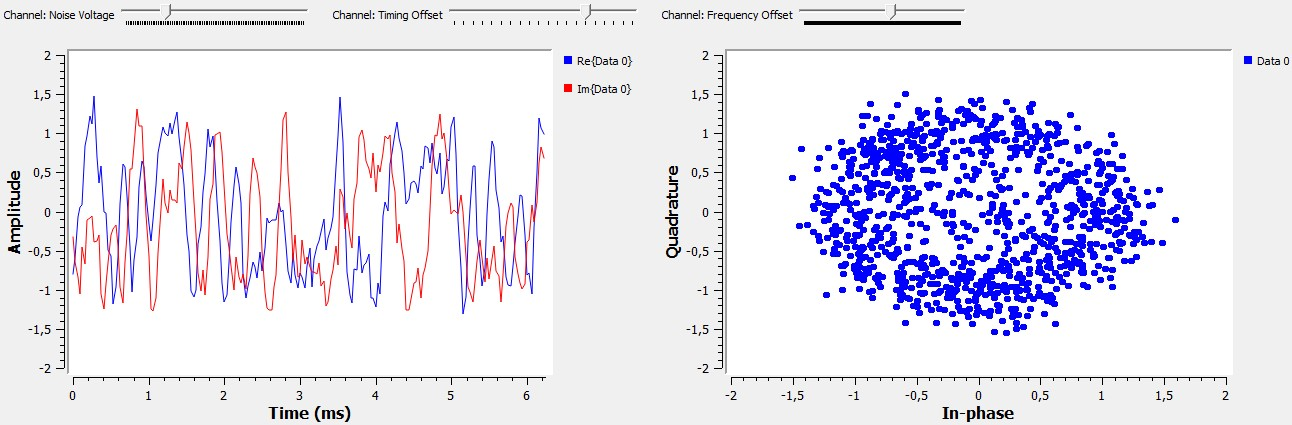
\includegraphics[width=1.0\textwidth]{8.jpg}
		\caption{Смещение по времени и фазе}
		\label{fig:8}
	\end{figure}
	\begin{figure}[H]
		\centering
		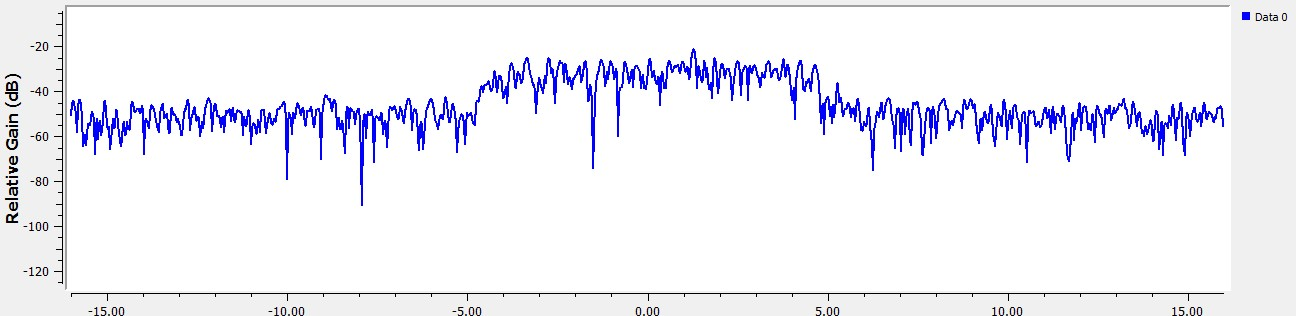
\includegraphics[width=1.0\textwidth]{9.jpg}
		\caption{Смещение по частоте}
		\label{fig:9}
	\end{figure}
	График созвездия показывает нам облако выборок гораздо худшее, чем мы ожидали увидеть. В дальнейшем мы это исправим.
	
	\chapter{Синхронизация}
	Существует множество алгоритмов, которые можно использовать для восстановления эффектов на одном этапе или сразу на нескольких этапах одновременно. 
	
	Здесь мы воспользуемся алгоритмом полифазной синхронизации тактовых сигналов. 
	
	Для правильной коррекции времени нам надо найти лучшее время для выборки входящих сигналов, что позволит максимизировать отношение сигнала к шуму для каждой выборки и уменьшить влияние межсимвольных помех.
	
	На следующей диаграмме мы создаем 4 отдельных символа 1 в  строке, а затем используем фильтр.
	\begin{figure}[H]
		\centering
		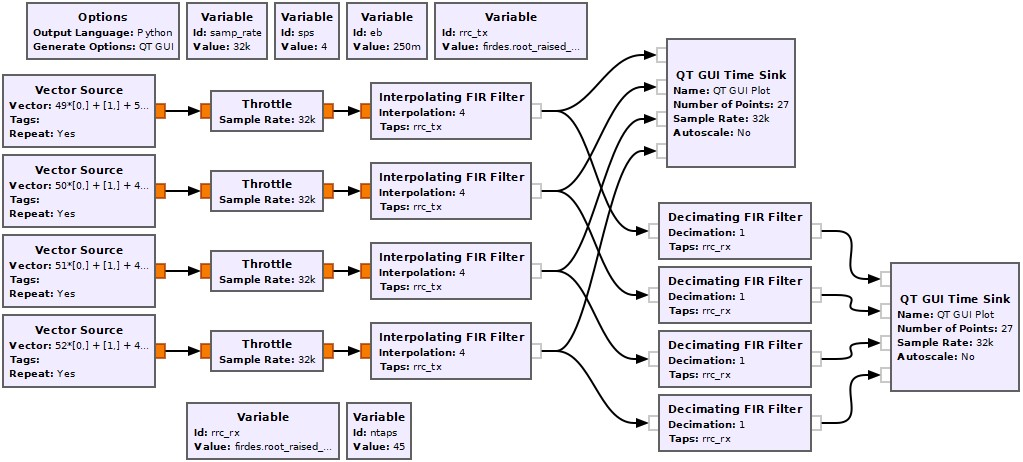
\includegraphics[width=1.0\textwidth]{10.jpg}
		\caption{Схема 4. \texttt{symbol\_sampling.grc}}
		\label{fig:10}
	\end{figure}
	\begin{figure}[H]
		\centering
		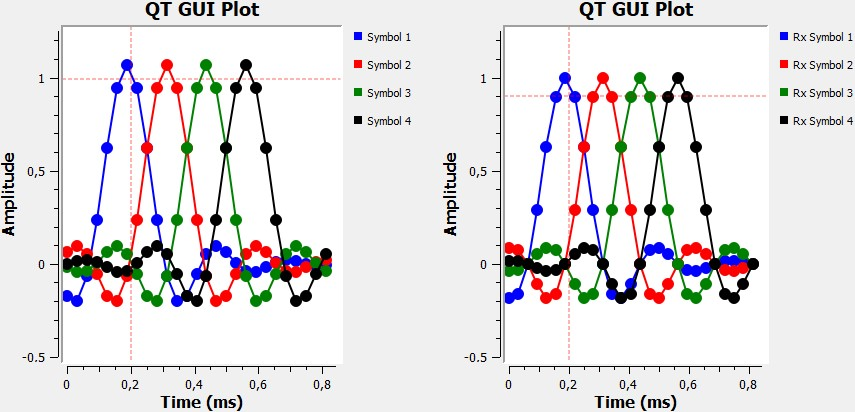
\includegraphics[width=1.0\textwidth]{11.jpg}
		\caption{Результаты работы 4-й схемы}
		\label{fig:11}
	\end{figure}
	Выходные данные показывают различия между символами \sloppy{\texttt{RRC}}- и \sloppy{\texttt{RC}}-фильтрации. Без фильтрации Найквиста мы можем видеть, как в идеальной точке выборки каждого символа другие символы обладают некоторой энергией. Если мы просуммируем эти символы вместе, энергия этих других выборок исказит символ в этой точке.
	
	И наоборот, на выходе \sloppy{\texttt{RC}}-фильтра энергия от других выборок равна 0 в идеальной точке выборки для данного символа. Это означает, что если мы выберем выборку точно в правильной точке выборки, мы получим энергию только от текущего символа без помех со стороны других символов в потоке.
	
	Это моделирование позволяет нам изменять количество выборок на символ и избыточную пропускную способность \sloppy{\texttt{RRC}}-фильтров.

	Посмотрим, что происходит из-за разной частоты тактовых сигналов, влияющих на точки выборки между передатчиком и приемником.
	
	Все тактовые сигналы не идеальны, и поэтому будут начинаться в любой момент времени и дрейфовать относительно других тактовых сигналов. Добавим в схему ресемплер (resampler), который регулирует частоту дискретизации символов в передаваемом сигнале.
	
	Разница в тактовых сигналах, показанная здесь, является завышенной для лучшей визуализации.
	\begin{figure}[H]
		\centering
		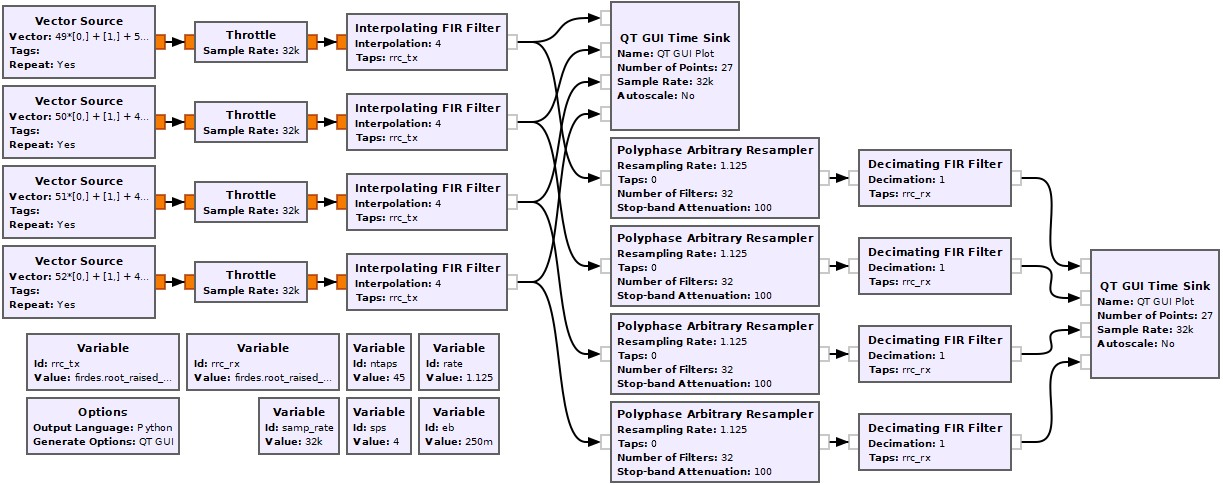
\includegraphics[width=1.0\textwidth]{12.jpg}
		\caption{Схема 5. \texttt{symbol\_sampling\_diff.grc}}
		\label{fig:12}
	\end{figure}
	\begin{figure}[H]
		\centering
		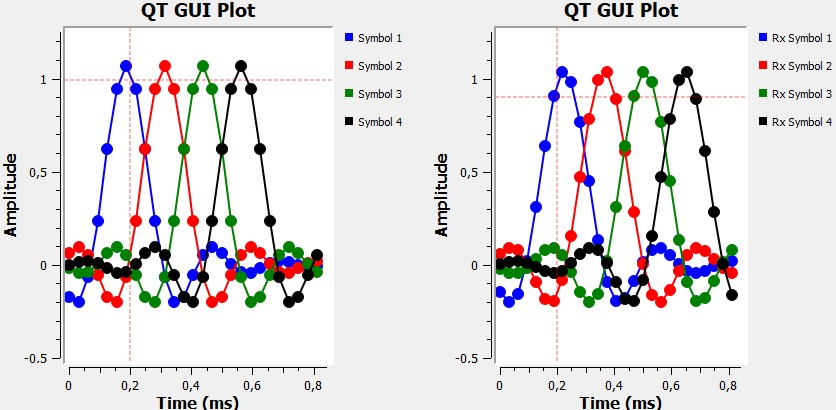
\includegraphics[width=1.0\textwidth]{13.jpg}
		\caption{Результаты работы 5-й схемы}
		\label{fig:13}
	\end{figure}
	Мы должны придумать способ, как синхронизировать тактовую частоту передатчика и приемника, используя только информацию, получаемую из передаваемого сигнала.

	\chapter{Небольшая информация о блоке полифазной синхронизации тактовых сигналов}
	Существует много разных алгоритмов, которые мы можем использовать для синхронизации тактового сигнала в приемнике. Все они включают в себя какой-то контур управления обратной связью. Мы будем использовать метод синхронизации тактовых импульсов с помощью полифазного фильтра (\sloppy{\texttt{polyphase filterbank}}). Этот блок предназначен для нескольких целей: синхронизация тактовых сигналов, фильтр приемника  (для уменьшения \sloppy{\texttt{ISI}} и дискретизация сигнала (1 выборка на символ).

	Блок работает путем вычисления первого дифференциала входящего сигнала, который будет связан со смещением его тактовой частоты. Когда выход дифференциального фильтра равен 0, мы нашли оптимальную точку выборки.
	\begin{figure}[H]
		\centering
		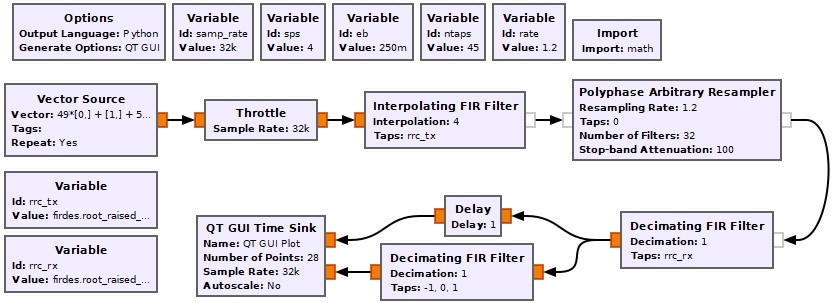
\includegraphics[width=1.0\textwidth]{14.jpg}
		\caption{Схема 6. \texttt{symbol\_differential\_filter.grc}}
		\label{fig:14}
	\end{figure}
	\begin{figure}[H]
		\centering
		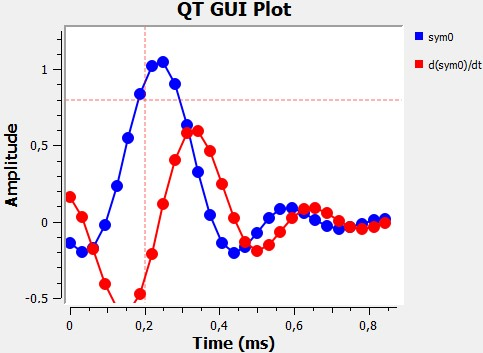
\includegraphics[width=0.75\textwidth]{15.jpg}
		\caption{\textquote{Идеальный} случай}
		\label{fig:15}
	\end{figure}
	Смещения времени нет, и график производной показывает точку на нуле.
	\begin{figure}[H]
		\centering
		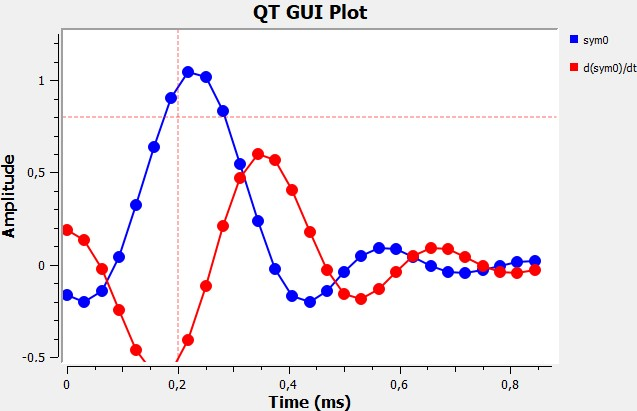
\includegraphics[width=0.75\textwidth]{16.jpg}
		\caption{Смещение по времени}
		\label{fig:16}
	\end{figure}
	Вместо использования одного фильтра мы можем создать серию фильтров, каждый из которых имел бы свою фазу. Если у нас будет достаточно фильтров на разных фазах, одна из них даст нам желаемое значение тактового сигнала.
	
	В следующей схеме используется 5 фильтров с 5 различными фазами.
	\begin{figure}[H]
		\centering
		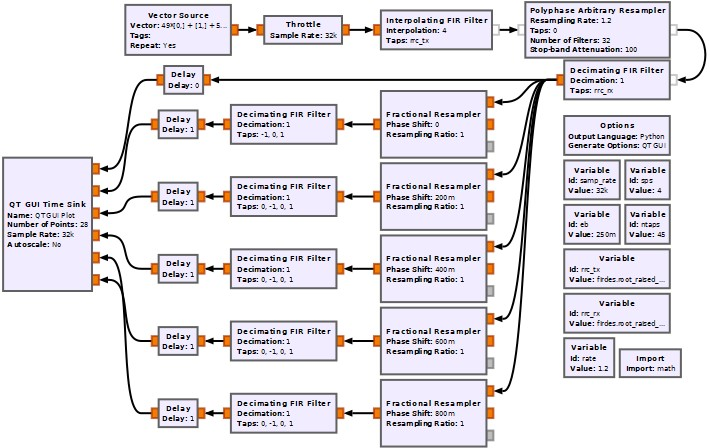
\includegraphics[width=1.0\textwidth]{17.jpg}
		\caption{Схема 7. \texttt{symbol\_differential\_filter\_phases.grc}}
		\label{fig:17}
	\end{figure}
	\begin{figure}[H]
		\centering
		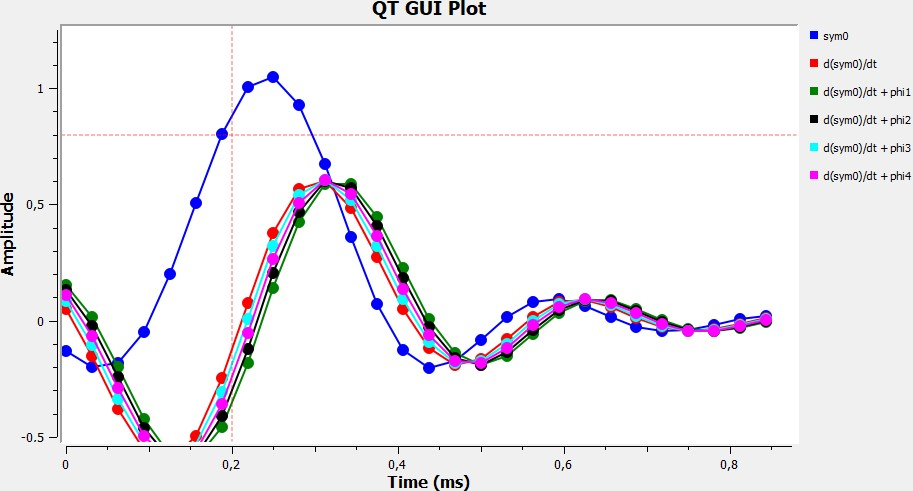
\includegraphics[width=1.0\textwidth]{18.jpg}
		\caption{5 фильтров с 5 различными фазами}
		\label{fig:18}
	\end{figure}
	Мы видим, что сигнал, помеченный как $d(sym0)/dt + phi3$, имеет точку выборки в нуле. Идеальная точка выборки происходит при этом смещении фазы.

	Мы можем рассматривать эти различные фильтры как части одного большого фильтра. Проблема в том, что мы говорим о большой дополнительной вычислительной сложности, поскольку она пропорциональна нашей частоте дискретизации. Вместо этого мы работаем с фильтрами разных фаз на входящей частоте дискретизации.

	Сигнал ошибки для синхронизации тактовых сигналов является выходом дифференциального фильтра. Контур управления начинается с одного из фильтров и вычисляет выходной сигнал как сигнал ошибки. Затем он перемещается вверх или вниз по ряду фильтров пропорционально сигналу ошибки до момента, где этот сигнал ошибки ближе всего к 0. И поскольку мы ожидаем, что тактовые сигналы передатчика и приемника будут дрейфовать относительно друг друга, мы можем воспользоваться контуром управления второго порядка для получения как правильной фазы фильтра, так и разности фаз между тактовыми сигналами.

	Запустим сценарий для исследования поведения блока восстановления полифазной синхронизации тактовых сигналов.
	\begin{figure}[H]
		\centering
		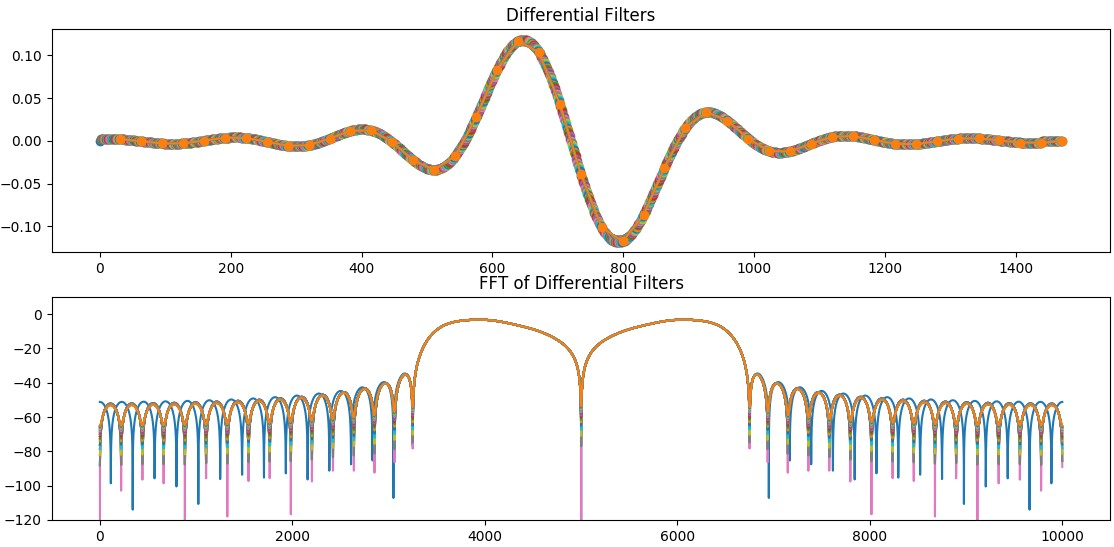
\includegraphics[width=1.0\textwidth]{19.jpg}
		\caption{Результаты работы Схемы 8. \texttt{example\_timing.py}}
		\label{fig:19}
	\end{figure}
	\begin{figure}[H]
		\centering
		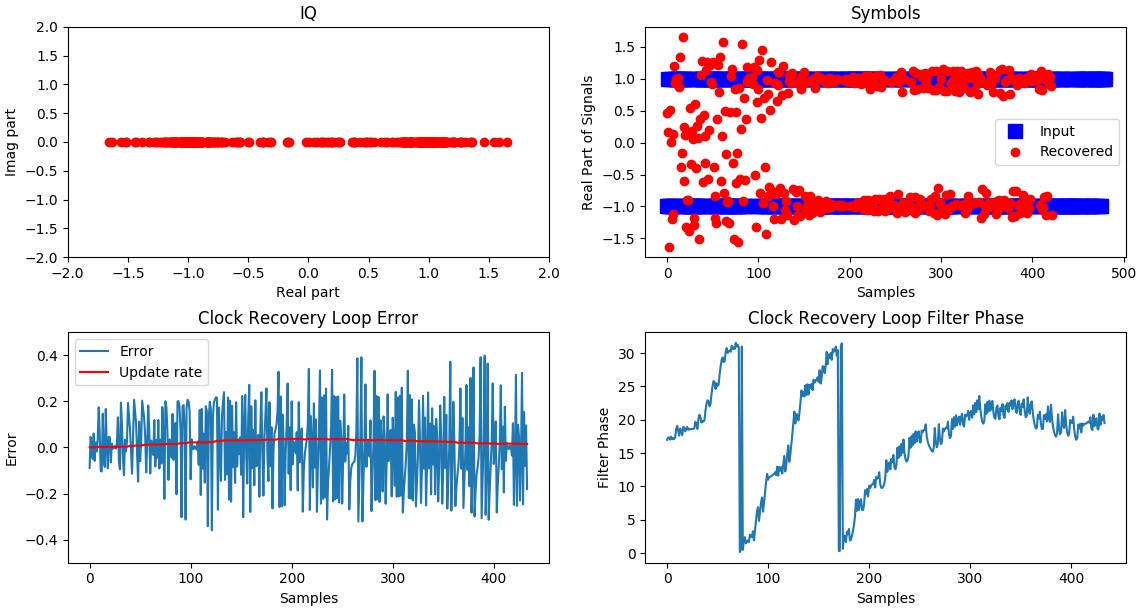
\includegraphics[width=1.0\textwidth]{20.jpg}
		\caption{Результат синхронизации тактовых сигналов}
		\label{fig:20}
	\end{figure}
	
	\chapter{Использование полифазного блока синхронизации тактовых сигналов в приемнике}
	Блок полифазной синхронизации тактовых сигналов настроен на 32 фильтра и пропускной способностью цикла $\frac{2 \pi}{100}$. Этот блок будет адаптироваться к ожидаемому значению выборок в зависимости от скорости входящего сигнала.
	\begin{figure}[H]
		\centering
		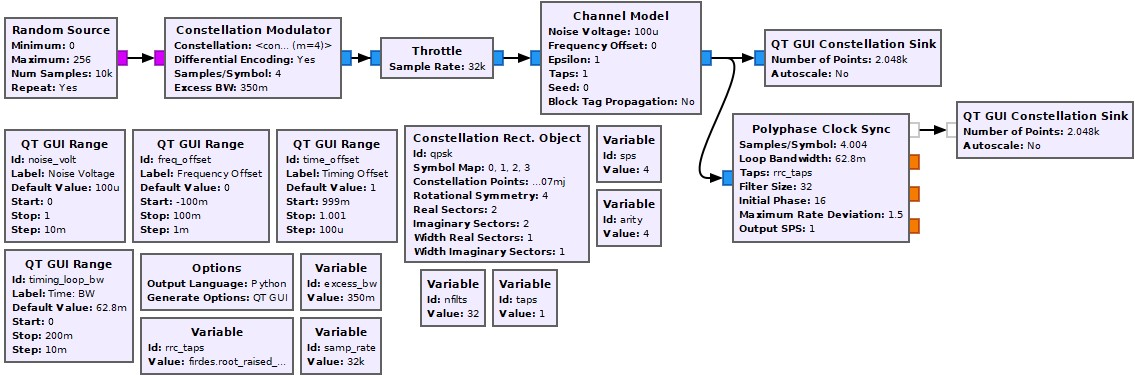
\includegraphics[width=1.0\textwidth]{21.jpg}
		\caption{Схема 9. \texttt{mpsk\_stage3.grc}}
		\label{fig:21}
	\end{figure}
	\begin{figure}[H]
		\centering
		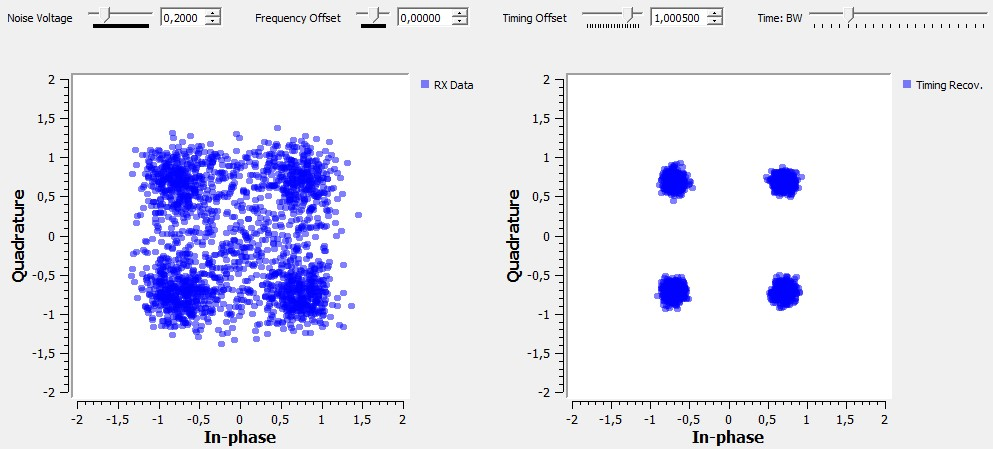
\includegraphics[width=1.0\textwidth]{22.jpg}
		\caption{Результат при запуске схемы}
		\label{fig:22}
	\end{figure}
	При запуске этого скрипта мы видим созвездие слева как принятый сигнал до восстановления синхронизации, а справа - после восстановления синхронизации.
	
	Изменение временной шкалы показывает нам, как блок синхронизации тактовых сигналов удерживает сигнал во времени и выводит выборки в идеальных точках созвездия. Если мы добавим смещение частоты, то увидим, что созвездие становится кругом.
	
	Созвездие находится на единичном круге, но блок не позволяет нам корректировать смещение частоты.
	\begin{figure}[H]
		\centering
		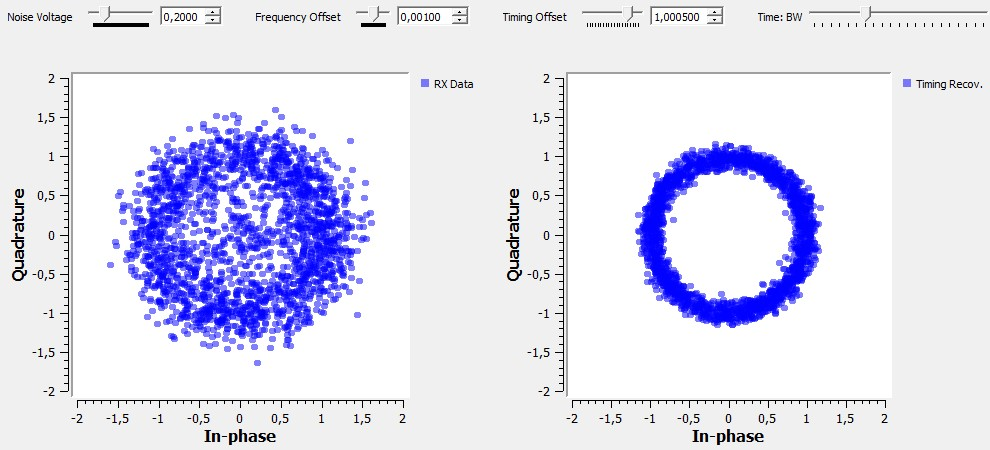
\includegraphics[width=1.0\textwidth]{23.jpg}
		\caption{Круговое созвездие}
		\label{fig:23}
	\end{figure}
	
	\chapter{Канал с несколькими путями}
	Канал с несколькими путями является результатом того, что в большинстве коммуникационных сред у нас нет единого пути для передачи сигнала от передатчика к приемнику. Каждый раз, когда появляется объект, отражающий сигнал, между двумя узлами может быть установлен новый путь. Каждый из этих отраженных сигналов будет отображаться в приемнике в разное время в зависимости от длины пути. Суммирование их вместе в приемнике вызовет искажения, как конструктивные, так и деструктивные.

	Влияние комбинации этих сигналов на приемник заключается в искажении сигнала. Если разница во времени между отражениями достаточно мала относительно ширины символа, искажение может быть внутри символа. Когда отражения длиннее, отражение от одного символа повлияет на следующие сигналы.

	Нам нужно исправить это поведение, например, с помощью блока, очень похожего на стерео-эквалайзер. С помощью стерео-эквалайзера мы можем изменить усиление определенных частот, чтобы либо подавить, либо усилить отражённые сигналы.
	\begin{figure}[H]
		\centering
		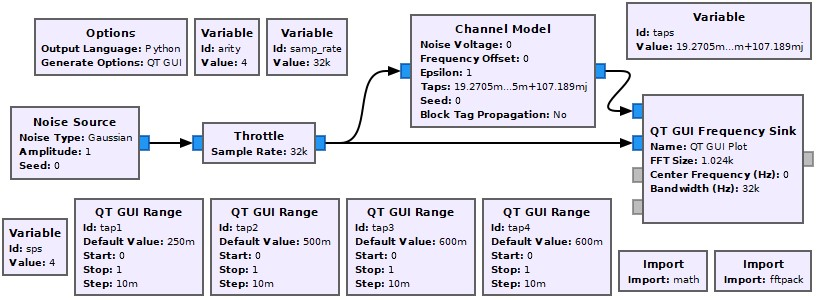
\includegraphics[width=1.0\textwidth]{24.jpg}
		\caption{Схема 10. \texttt{multipath\_sim.grc}}
		\label{fig:24}
	\end{figure}
	Это моделирование настраивает модель канала с 4  управляемыми параметрами. Эти элементы управления настроены одинаково по частоте, и мы можем настроить их от 0 до 1. При значении 1 частоты смогут проходить без помех. При значении 0 они создадут \textquote{глубокий нуль} в спектре, который повлияет на все частоты вокруг него.
	\begin{figure}[H]
		\centering
		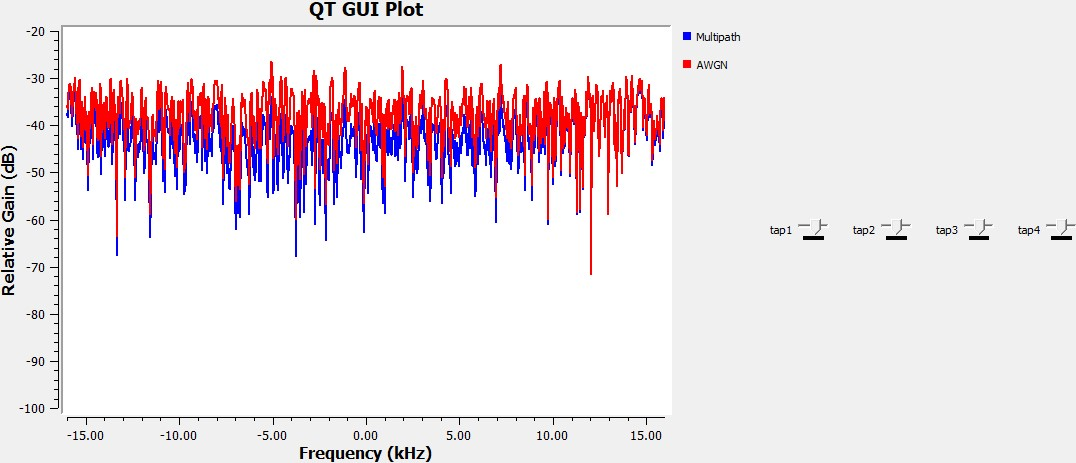
\includegraphics[width=1.0\textwidth]{25.jpg}
		\caption{Средние значения параметров}
		\label{fig:25}
	\end{figure}
	\begin{figure}[H]
		\centering
		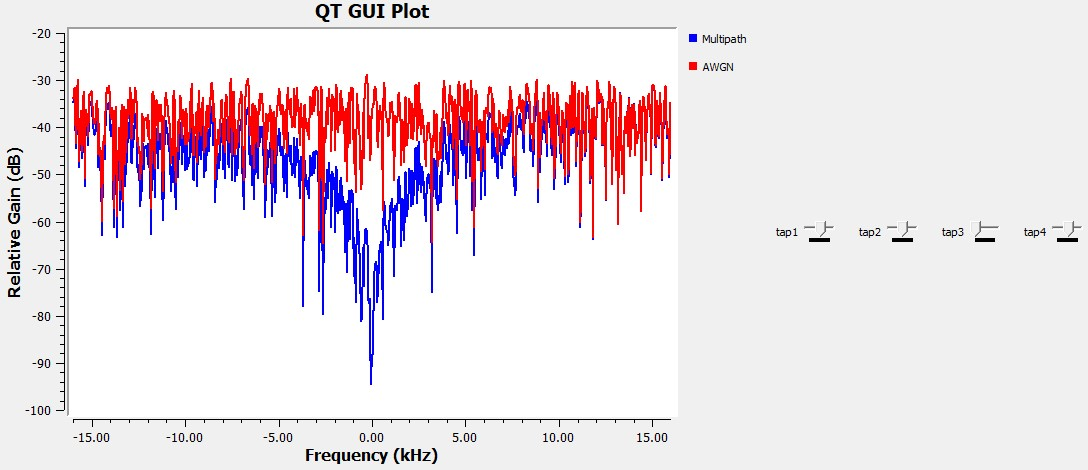
\includegraphics[width=1.0\textwidth]{26.jpg}
		\caption{\textquote{Глубокий нуль}}
		\label{fig:26}
	\end{figure}

	\chapter{Эквалайзеры}
	Задача эквалайзера - инвертировать канал передачи сигнала. Наша цель сделать так, чтобы искаженный принятый сигнал отражался снова как плоский. Для этого надо найти правильный алгоритм эквалайзера и настроить его параметры.

	Есть два вида эквалайзеров: эквалайзер \sloppy{\texttt{CMA}} и эквалайзер \sloppy{\texttt{LMS DD}}. \sloppy{\texttt{CMA}}, или Алгоритм с постоянным модулем, является \textquote{слепым} эквалайзером и работает только с сигналами, имеющими постоянную амплитуду. Это означает, что цифровые сигналы, такие как \sloppy{\texttt{MPSK}}, хорошо подходят для этого алгоритма, поскольку они имеют точки только на единичном круге.
	\begin{figure}[H]
		\centering
		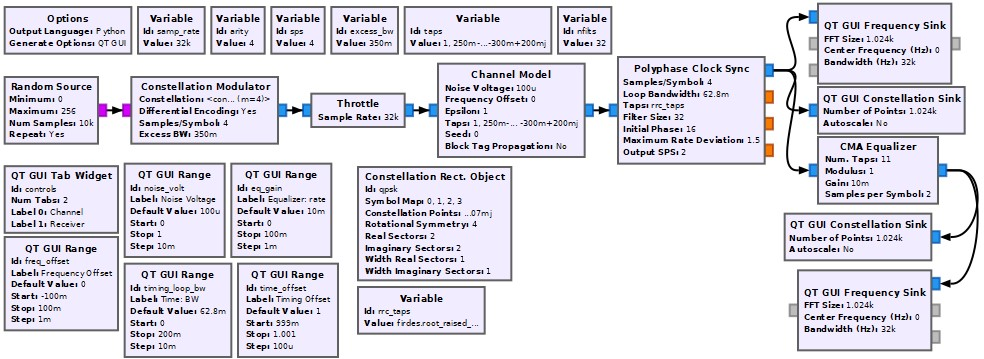
\includegraphics[width=1.0\textwidth]{27.jpg}
		\caption{Схема 11. \texttt{mpsk\_stage4}. Первая версия}
		\label{fig:27}
	\end{figure}
	Мы можем наблюдать, как алгоритм \sloppy{\texttt{CMA}} сходится. Также, поскольку у нас есть как синхронизация тактовых сигналов, так и блок эквалайзера, они сходятся независимо, но один этап повлияет на следующий этап. Таким образом, здесь происходит некоторое взаимодействие между последовательными этапами.
	
	Перед эквалайзером у нас очень странный сигнал, и эквалайзер понимает, как его сделать чистым. Мы также можем видеть сам канал и то, как он хорошо выравнивается после эквалайзера.
	\begin{figure}[H]
		\centering
		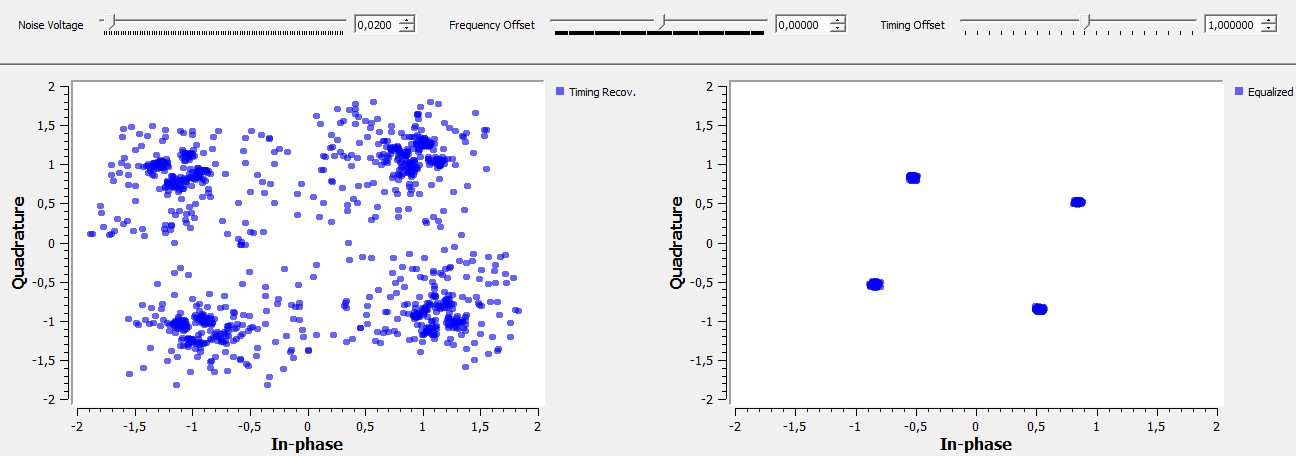
\includegraphics[width=1.0\textwidth]{28.jpg}
		\caption{Смещение по фазе}
		\label{fig:28}
	\end{figure}
	\begin{figure}[H]
		\centering
		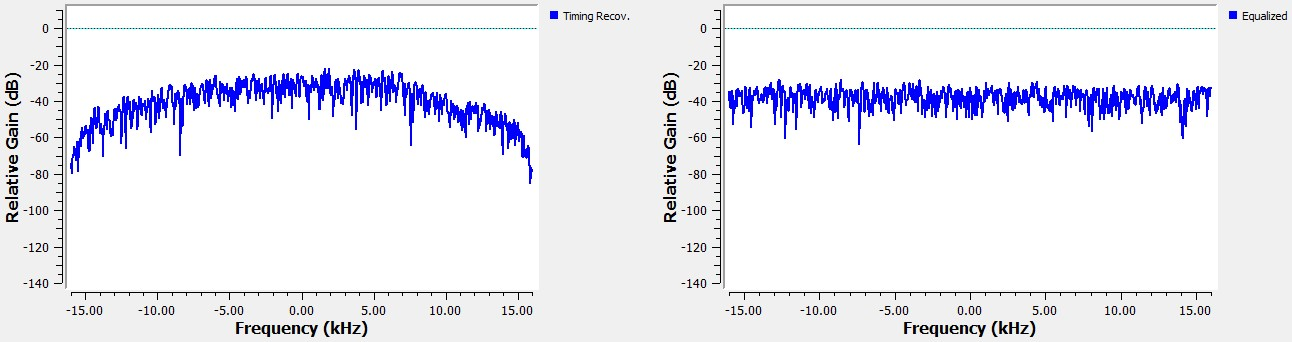
\includegraphics[width=1.0\textwidth]{29.jpg}
		\caption{Смещение по частоте}
		\label{fig:29}
	\end{figure}
	Изменили значения некоторых параметров эквалайзера и получили немного другие результаты:
	\begin{figure}[H]
		\centering
		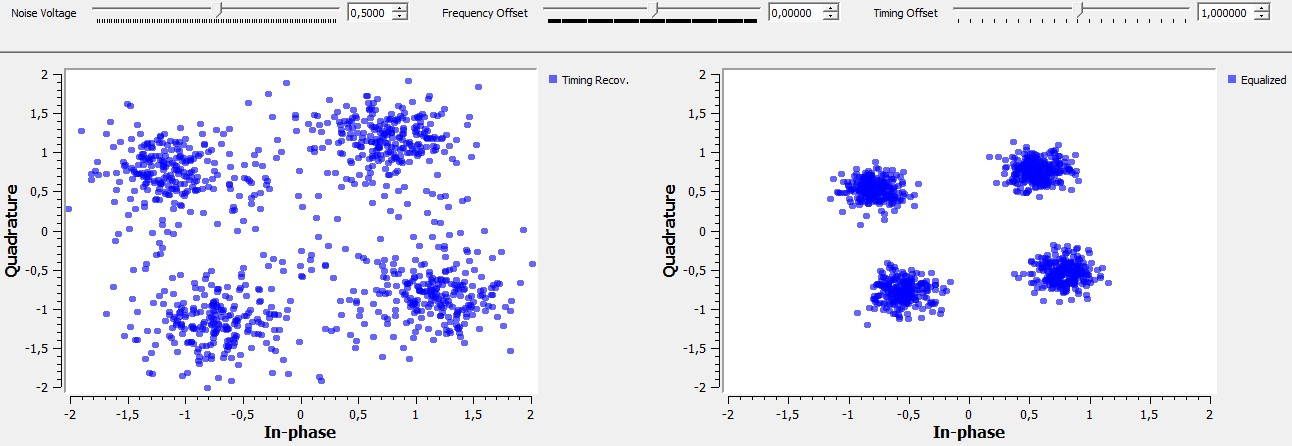
\includegraphics[width=1.0\textwidth]{30.jpg}
		\caption{Смещение по фазе с новыми параметрами}
		\label{fig:31}
	\end{figure}
	\begin{figure}[H]
		\centering
		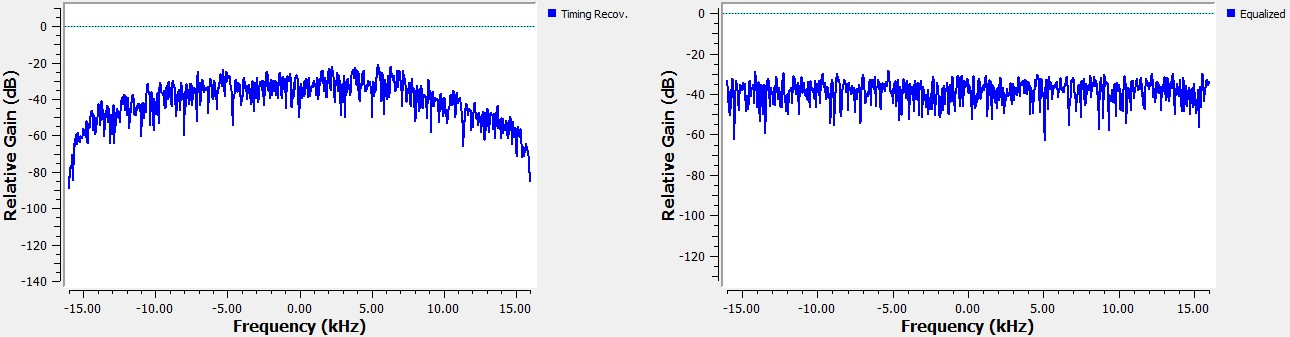
\includegraphics[width=1.0\textwidth]{31.jpg}
		\caption{Смещение по частоте с новыми параметрами}
		\label{fig:31}
	\end{figure}
	
	\chapter{LMS-DD Эквалайзер}
	Попробуем применить \sloppy{\texttt{LMS-DD}} эквалайзер (наименьший квадрат ошибки). Многие параметры совпадают с \sloppy{\texttt{CMA}} эквалайзером, но этому эквалайзеру требуется дополнительная информация о сигнале в виде точек созвездия.
	 
	Этот эквалайзер хорошо подходит для сигналов, которые не подходят под требование постоянной амплитуды, поэтому его можно использовать и для \sloppy{\texttt{QAM}}-модуляции. С другой стороны, если в канале большой шум, принимаемые эквалайзером решения могут быть некорректными, что заметно снизит производительность приемника. Однако, если сигнал хороший, то \sloppy{\texttt{LMS-DD}} эквалайзер может выдать заметно более хороший результат. Часто сначала используют слепой эквалайзер, когда мало информации о сигнале, а потом переключаются на \sloppy{\texttt{LMS-DD}}.
	\begin{figure}[H]
		\centering
		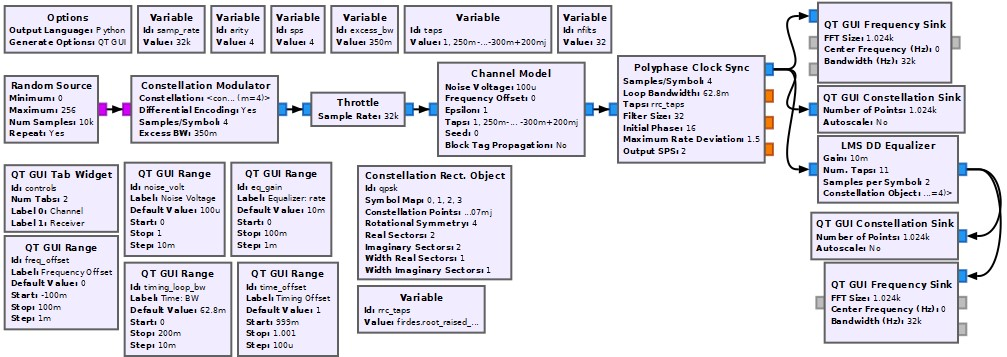
\includegraphics[width=1.0\textwidth]{32.jpg}
		\caption{Схема 12. \texttt{mpsk\_stage4}. Вторая версия}
		\label{fig:32}
	\end{figure}
	\begin{figure}[H]
		\centering
		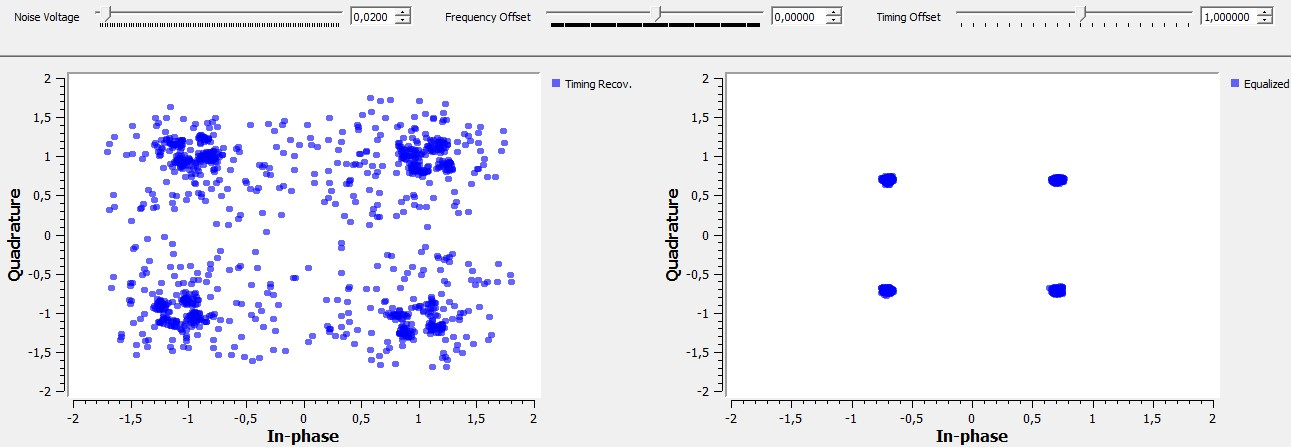
\includegraphics[width=1.0\textwidth]{33.jpg}
		\caption{Смещение по фазе}
		\label{fig:33}
	\end{figure}
	\begin{figure}[H]
		\centering
		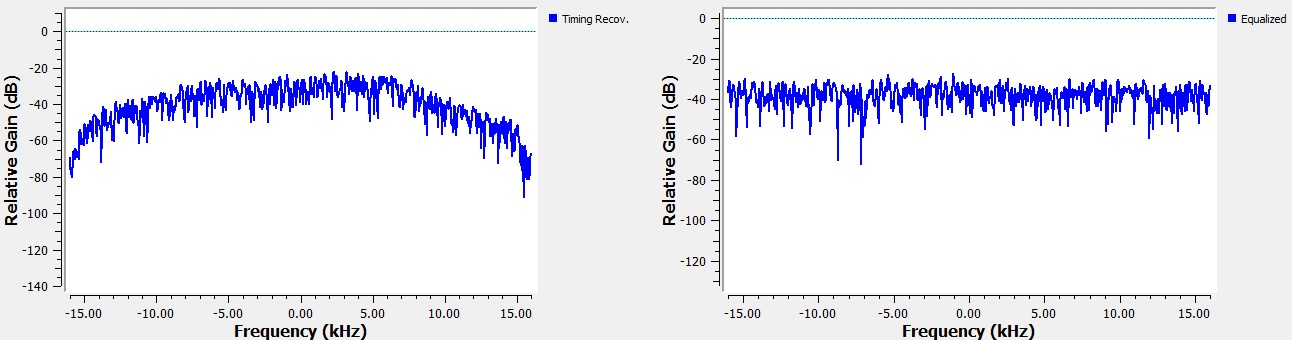
\includegraphics[width=1.0\textwidth]{34.jpg}
		\caption{Смещение по частоте}
		\label{fig:34}
	\end{figure}
	Снова изменили значения некоторых параметров эквалайзера и получили другие результаты:
	\begin{figure}[H]
		\centering
		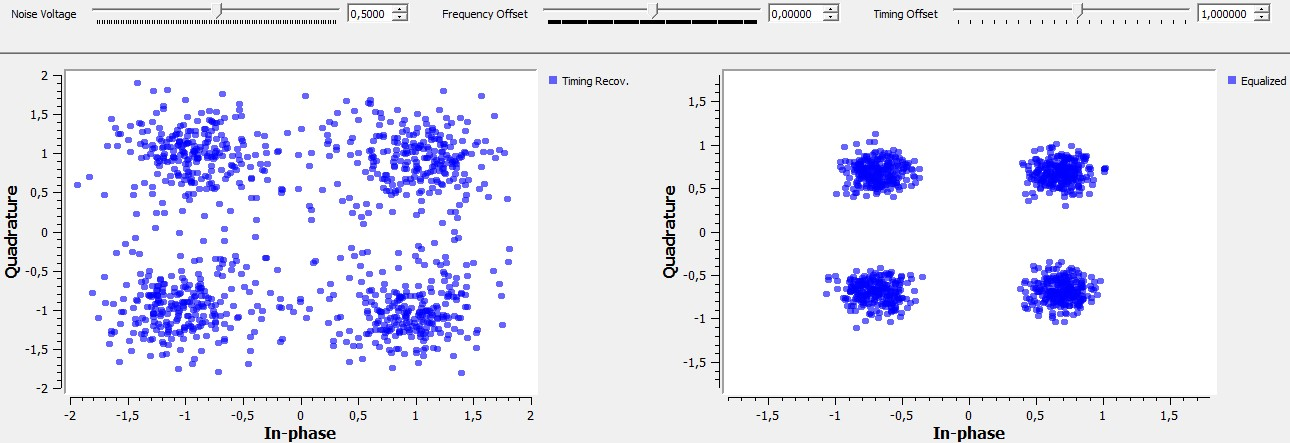
\includegraphics[width=1.0\textwidth]{35.jpg}
		\caption{Смещение по фазе с новыми параметрами}
		\label{fig:35}
	\end{figure}
	\begin{figure}[H]
		\centering
		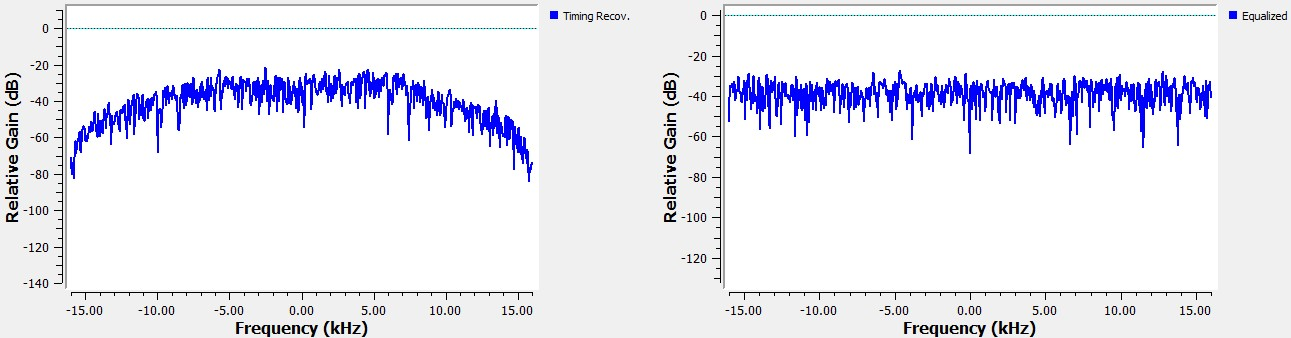
\includegraphics[width=1.0\textwidth]{36.jpg}
		\caption{Смещение по частоте с новыми параметрами}
		\label{fig:36}
	\end{figure}
	Результаты работы двух разных эквалайзеров совпали (визуально).
	
	\chapter{Коррекция по частоте и фазе}
	После применения эквалайзера у нас все еще остались проблемы со смещением фазы и частоты. Эквалайзеры, как правило, не адаптируются быстро, и поэтому смещение частоты может быть за пределами возможностей эквалайзера. Кроме того, \sloppy{\texttt{CMA}} эквалайзер ничего не знает о созвездии, поэтому могут возникнуть проблемы с выбором начальной фазы для точки отсчета.

	На этой стадии мы будем использовать цикл второго порядка, чтобы мы могли отслеживать как фазу, так и частоту (которая является производной от фазы) с течением времени. Тип восстановления, с которым мы будет здесь работать, предполагает, что мы выполняем точную частотную коррекцию. Поэтому мы должны быть уверены, что уже находимся близко к идеальной частоте. Если мы будем слишком далеко,  цикл не сойдется. 

	Для этой задачи мы воспользуемся циклом Костаса. Соответствующий блок может синхронизировать \sloppy{\texttt{BPSK}}, \sloppy{\texttt{QPSK}} и \sloppy{\texttt{8PSK}}.
	\begin{figure}[H]
		\centering
		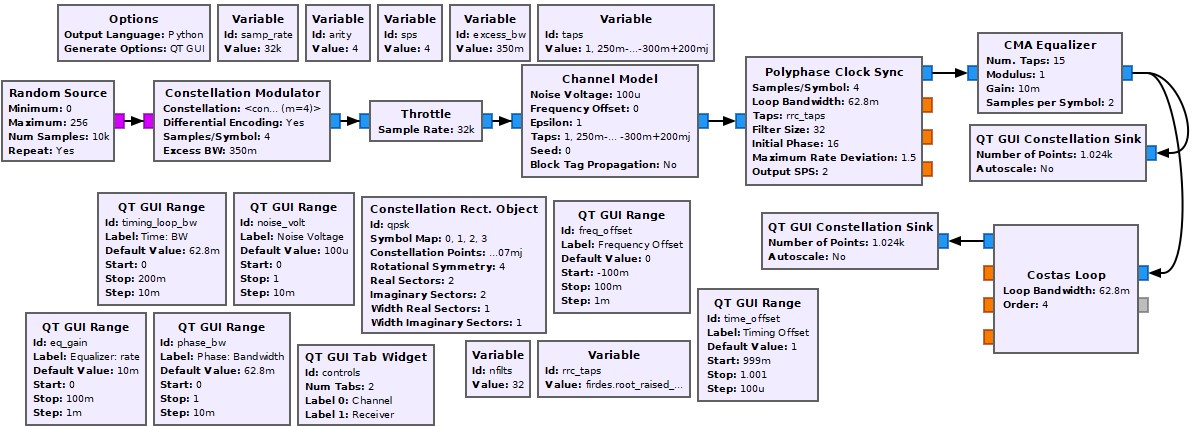
\includegraphics[width=1.0\textwidth]{37.jpg}
		\caption{Схема 13. \texttt{mpsk\_stage5.grc}}
		\label{fig:37}
	\end{figure}
	Этот блок, как и все другие, использует цикл второго порядка и поэтому определяется параметром пропускной способности. Он должен знать порядок модуляции \sloppy{\texttt{PSK}}: 2 для \sloppy{\texttt{BPSK}}, 4 для \sloppy{\texttt{QPSK}} и 8 для \sloppy{\texttt{8PSK}}. 
	После работы эквалайзера мы видим, что все символы находятся на единичном круге, но вращаются из-за смещения частоты, которое мы ещё не исправили. На выходе цикла Костаса мы видим созвездие, похожее на исходное, но с дополнительным шумом, с которым мы ничего не можем поделать.
	\begin{figure}[H]
		\centering
		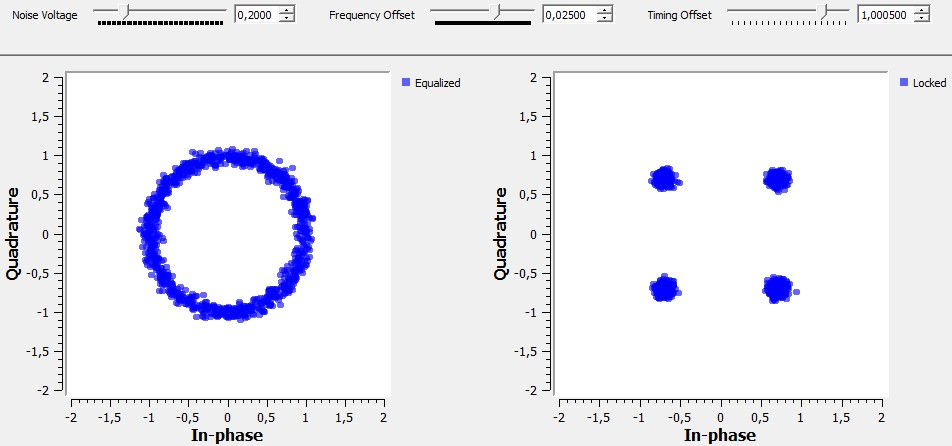
\includegraphics[width=1.0\textwidth]{38.jpg}
		\caption{Результат работы 13-й схемы}
		\label{fig:38}
	\end{figure}
	
	\chapter{Декодер}
	Теперь, когда сложная часть уже пройдена, мы приступаем к декодированию сигнала. Добавляем Декодер созвездий (Constellation Decoder) после цикла Костаса. 
	
	На этом этапе мы получаем наши символы от 0 до 3, потому что это размер нашего алфавита в схеме \sloppy{\texttt{QPSK}}. У нас нет никакой уверенности, что эти символы правильно передаются. Раньше мы обходили эту проблему, передавая дифференциальные символы. На самом деле мы передавали не само созвездие, а разницу между символами созвездия, установив дифференциальную настройку в блоке \textquote{Constellation Modulator} в значение \sloppy{\texttt{Yes}}. Уберем этот флажок.
	\begin{figure}[H]
		\centering
		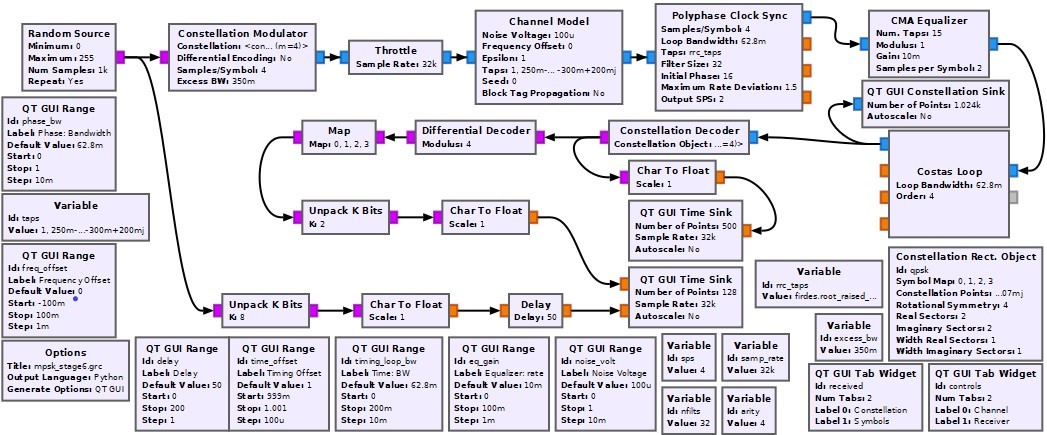
\includegraphics[width=1.0\textwidth]{39.jpg}
		\caption{Схема 14. \texttt{mpsk\_stage6.grc}. Первая версия}
		\label{fig:39}
	\end{figure}
	Cхема использует блок дифференциального декодера (Differential Decoder) для перевода дифференциально закодированных символов обратно в исходные символы с помощью сдвигов фаз, а не самой абсолютной фазы. Но даже так наши символы не совсем верны. На самом деле это самая трудная часть демодуляции. На этапах синхронизации на нашей стороне были основы физики и математики. Теперь мы должны интерпретировать какой-то символ, основываясь лишь на том, как его описал другой.  Мы используем блок карты (Map) для преобразования символов из дифференциального декодера в исходные символы, которые мы передали. На данный момент у нас теперь есть исходные символы от 0 до 3, поэтому распакуем эти 2 бита в символе в отдельные биты с помощью блока \sloppy{\texttt{Unpack Bit}}.

	Чтобы убедиться в правильности передачи, сравним выходной поток с входным битовым потоком. Передатчик произвел упакованные биты, поэтому мы снова используем \sloppy{\texttt{Unpack Bit}} для распаковки с 8 бит на байт до 1 бита на байт. Затем мы преобразуем эти потоки в значения с плавающей запятой 0.0 и 1.0 просто потому, что \sloppy{\texttt{Time Sink}} принимают только значения с плавающей запятой и комплексные значения. Напрямую сравнивать значения нельзя, поскольку цепочка приемника имеет много блоков и фильтров, которые задерживают сигнал, поэтому принятый сигнал отстает на некоторое количество битов. Чтобы компенсировать это, мы должны задержать передаваемые биты на ту же величину, используя блок \sloppy{\texttt{Delay}}. 
	
	\begin{figure}[H]
		\centering
		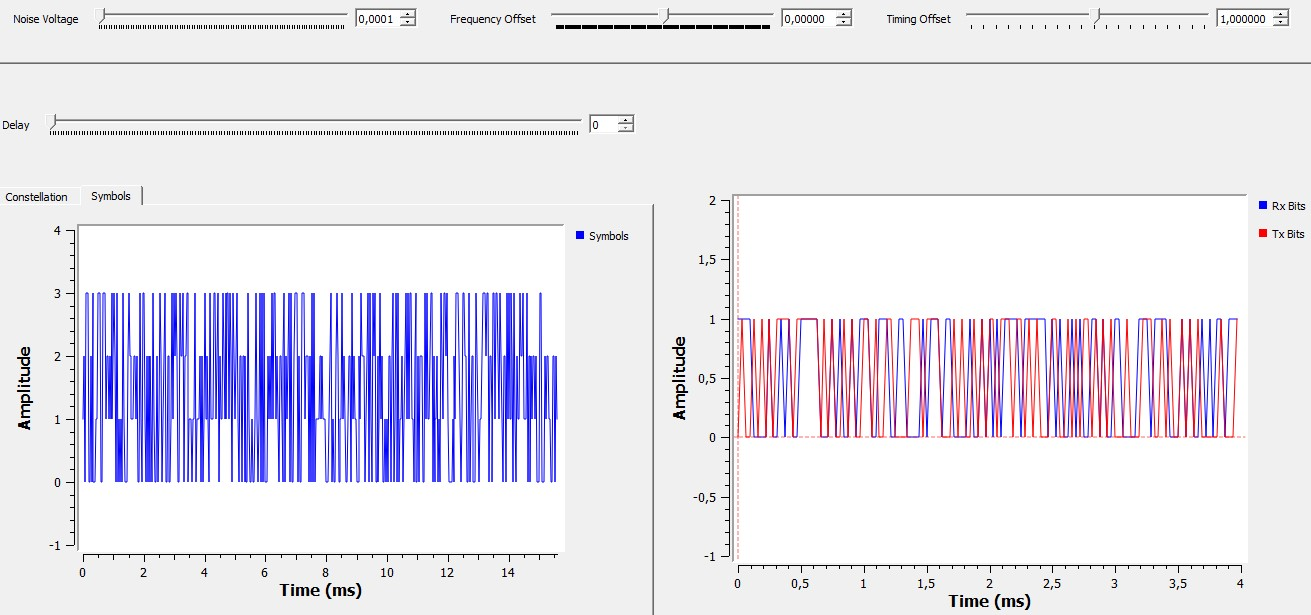
\includegraphics[width=1.0\textwidth]{40.jpg}
		\caption{Задержка настроена неправильно}
		\label{fig:40}
	\end{figure}
	Настроили задержку, чтобы найти правильное значение для синхронизизации бит.
	\begin{figure}[H]
		\centering
		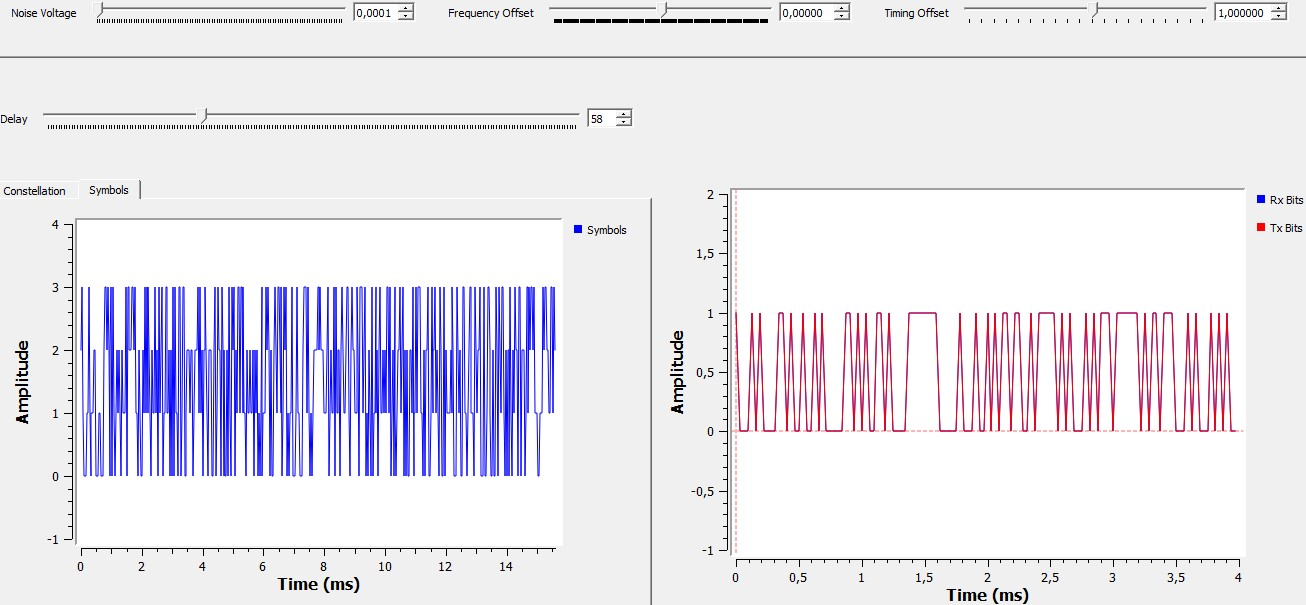
\includegraphics[width=1.0\textwidth]{41.jpg}
		\caption{Так уже лучше}
		\label{fig:41}
	\end{figure}
	Немного изменили схему, чтобы вычесть один сигнал из другого и увидеть, что выход будет равен 0. Добавление шума и других воздействий на канал может быть легко замечено как битовые ошибки, когда этот сигнал не равен 0.
	
	Мы используем генератор случайных чисел конечной длины, поэтому мы можем увидеть закономерность в принимаемом сигнале. Для этой цели воспользуемся блоком \sloppy{\texttt{QT GUI Time Raster Sink}}.
	\begin{figure}[H]
		\centering
		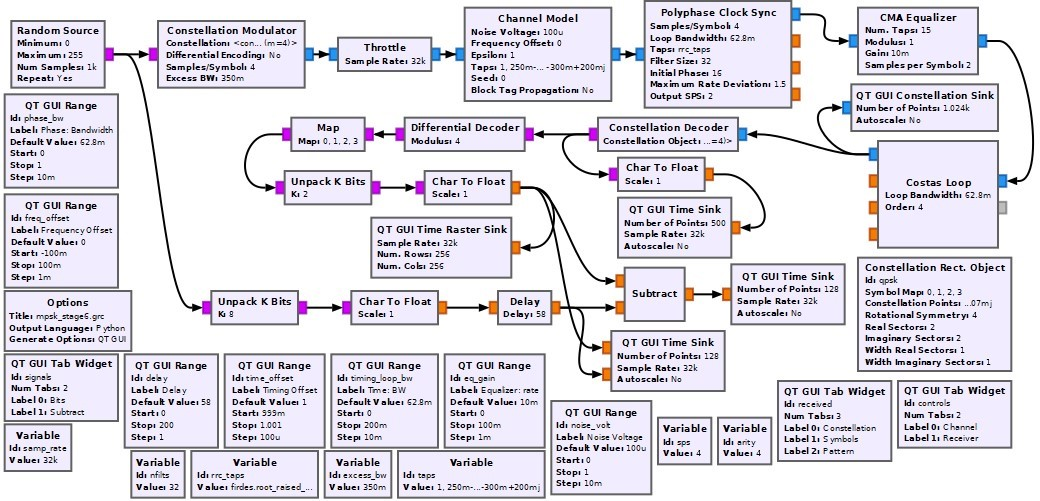
\includegraphics[width=1.0\textwidth]{43.jpg}
		\caption{Схема 15. \texttt{mpsk\_stage6.grc}. Вторая версия}
		\label{fig:43}
	\end{figure}
	\begin{figure}[H]
		\centering
		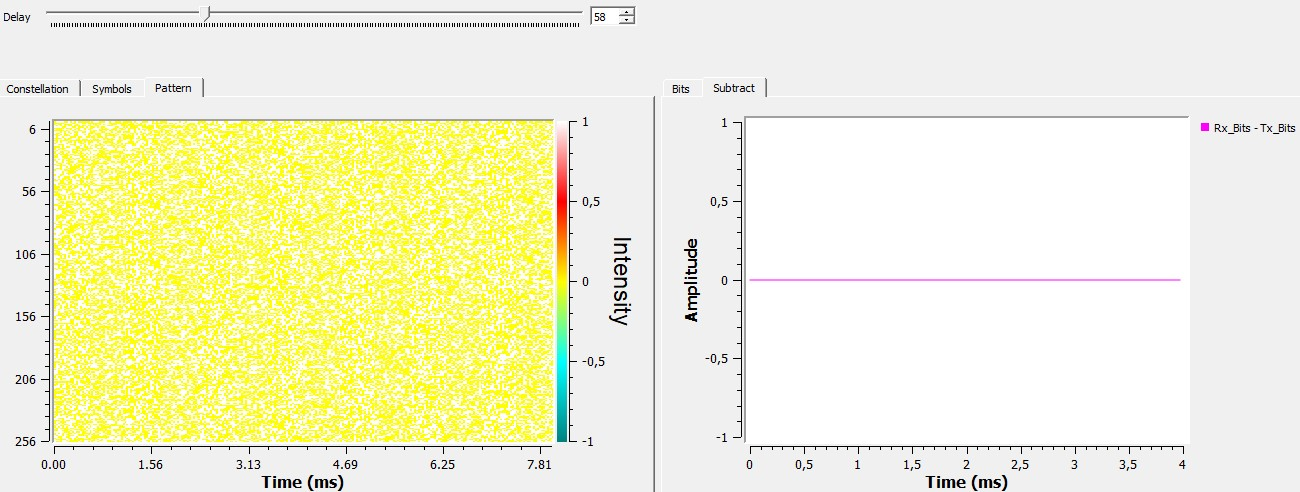
\includegraphics[width=1.0\textwidth]{42.jpg}
		\caption{Шаблон принимаемого сигнала}
		\label{fig:42}
	\end{figure}

	\chapter{Вывод}
	В данной работе мы рассмотрели множество интересных явлений, связанных с передачей сигналов. Симулируя настоящие условия передачи данных (например, шум), мы столкнулись с рядом трудностей и рассмотрели возможные пути их решения. Это поможет нам в будущем при организации настоящих каналов передачи различной информации.
\end{document}